\section{The graveyard, and the two laws it obeys}
\label{sec:laws}

Negative results are reported with the same protocol as positive
ones, because the map of what fails is half the deliverable.
Table~\ref{tab:graveyard} lists every rejected design with its
verdict statistic; each has a full module report with its
pre-registration in the repository. The pattern is not random.

\paragraph{Law 1: states have no arrow.} Fifteen crowding and
ownership-state formulations --- days-of-ADV held (level and its
published value-weighted point, which replicates raw and dies
residualized), ownership share, holder concentration, institutional
ownership changes at one and two quarters, breadth level, factor
crowding from manager tilts (three hypotheses), co-ownership graph
diffusion, flow-vulnerability centrality, forced-sale absorption and
overhang, latent-strategy crowding, and the aggregate stress index
against future returns --- carry no directional information. States
earned exactly two jobs in the production stack: denominators (ADV,
AUM) and risk conditioning (the deleveraging index against future
volatility). The one crowding-adjacent object that pays, FSS, is not
a state: it is a forced action divided by liquidity.

\paragraph{Law 2: distress is information when observed, never when
predicted.} Contemporaneous: $t\approx+10$ selling contrast, the FSS
regime short, the anti-panic monitor. Predictive: quarterly flow
forecasting dead at its mechanism gate; daily stress anticipation
retracted; crash cascades gated; exhaustion longs dead. Both clocks,
both directions, one conclusion --- and it implies the production
design: react fast to filings, do not front-run them.

\begin{figure}[t]
\centering
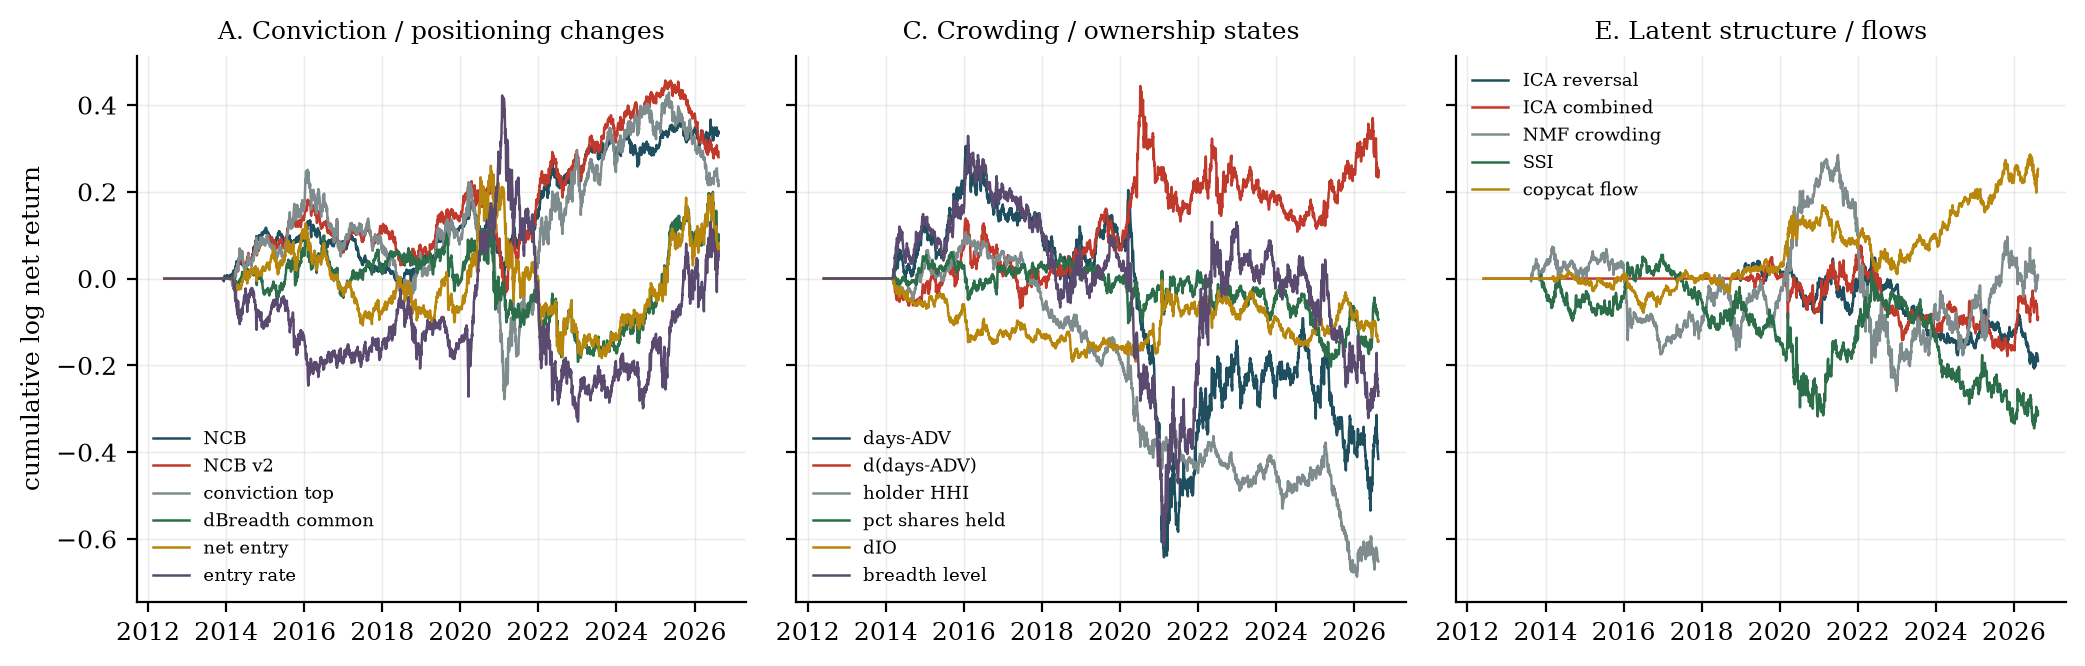
\includegraphics[width=\linewidth]{figs/f3_class_curves.png}
\caption{Net engine curves by signal class (log cumulative). The
conviction class carries the performance; the state class oscillates
around zero for a decade; the latent-structure class validates as
measurement but earns nothing net.}
\label{fig:classes}
\end{figure}

\paragraph{The smart-money corollary.} Nine designs weighting
managers by past performance or filtering the universe by manager
quality returned zero, and the base rates of
Section~\ref{sec:funds} say why: skill persistence of $0.25$ is too
weak to select on, and manager performance rank is approximately
orthogonal to \emph{which stocks} managers hold, so reweighting the
electorate reweights at random.

\begin{table}[t]
\centering\scriptsize
\caption{The graveyard. Every rejected design, its verdict statistic,
and its class. Full pre-registrations and reports in the repository
modules.}
\label{tab:graveyard}
\begin{tabular}{llll}
\toprule
design & class & verdict statistic & lesson \\
\midrule
performance-sigmoid vote weights & D & $t=+0.06$ & skill rank $\perp$ holdings \\
top-performer universes & D & negative & same \\
empirical-Bayes skill weights & D & negative & same \\
vol-scaled performance weights & D & negative & same \\
activity/concentration filters (U1--U4) & D & up to $t=-2.54$ & census beats filters \\
patient-manager universe & D & $t=-2.35/-3.25$ & same \\
follow-the-leader trading & B & hangover $t=-2.5$ & echo arrives late \\
five 13F$\times$classical interactions & A & none pass $2.57$ (5 tests) & signal is broad \\
pressure$\times$volatility (E4) & B & $t=+2.06\to+0.77$ & flicker died on fuller data \\
window dressing & F & both signs wrong & structure, not propensity \\
restatement direction-following & F & inverted ($t=-3.5$) & attention, not news \\
crash$\to$redemption cascade & B & gate $t=-1.47$ & 13F clock too coarse \\
funding-shock beta & C & $t=+0.77$, 2--3 episodes & not yet testable \\
exhaustion tactical long & F & thesis$-$placebo $t=+0.95$ & pressure continues \\
daily stress-anticipation short & F & \textbf{retracted} & eligibility artifact \\
correlation stress triggers & F & smoke mirage & Law: smoke never decides \\
cover-at-exhaustion & F & $-1.5\%$/q for 7 bps & hold the short \\
hot-ownership long warning & F & $t=+0.79$, wrong sign & --- \\
flow forecasting (stop-out prediction) & B & OOS rank-corr $-0.015$ & Law 2 \\
factor crowding as predictor & C & dead five ways & Law 1 \\
NMF strategy-crowding fragility & C & sign opposite thesis & Law 1 \\
ICA reversal as tradable & E & net $\approx 0$ & identification, not alpha \\
breadth level as factor & C & net Sharpe $-0.07$ & Law 1 \\
imbalance reversal (bias-adjusted) & F & premium shrinks & PIT accounting bites \\
ML nonlinear premium & A & boosted$-$ridge $t=+0.27$ & linear extracts it \\
\bottomrule
\end{tabular}
\end{table}
